% (c) 2019 Ben Crowell, licensed under the Creative Commons
% Attribution-ShareAlike license,
% http://creativecommons.org/licenses/by-sa/1.0/
%
\documentclass{lmseries}
% \let\ifpdf\relax % http://tex.stackexchange.com/questions/11414/package-ifpdf-error
% --------> this fails with TeX Live 2013, conflicts with xparse
%\selectlanguage{english}
\usepackage{lmlanguage}
%\includeonly{n1/ctemp}
\inputprotcode
\makeindex
\pdfmapfile{=fullembed.map} % created by the script create_fullembed_file
\begin{document}
\myeqnspacing % Do this early and often, since it gets reset by \normalsize
% 
% The following is all related to margin kerning.
% This is activated in dp.cls using the boolean wantmarginkerning.
% The constant 1 is to allow margin kerning, but to keep it from affecting
% line breaks.
\ifthenelse{\boolean{wantmarginkerning}}{
 \setprotcode\font
 {\it \setprotcode \font}
 {\bf \setprotcode \font}
 {\bf \it \setprotcode \font}
 \pdfprotrudechars=1
}{}
% Override lmcommon.cls, show subsection numbers:
\titleformat{\subsection}
  {\normalfont\normalsize\bfseries\sffamily\raggedright\protect\sansmath}{\showsecnum{\thesubsection}}{0.6em}{}   
% Override lmcommon.cls, no special label for calculus-based problems:
\renewcommand{\hwtopboilerplate}{%
  \noindent\formatlikesubsection{\langkey}\\*
  \begin{tabular}{lll}
    \hwcheckmark & A computerized answer check is available online. \\
    \displayhwdifficulty{2} & A difficult problem.
  \end{tabular}
}
%========================= frontmatter =========================
\formatchtoc{\Large}{}{4mm}
\frontmatter
\yesiwantarabic
\renewcommand{\chapdir}{front}
\begin{titlepages}
%
\thispagestyle{empty}
\raisebox{0mm}[0mm][0mm]{%
\parbox{8.5in}{
\vspace*{236mm}\hspace{-38.5mm}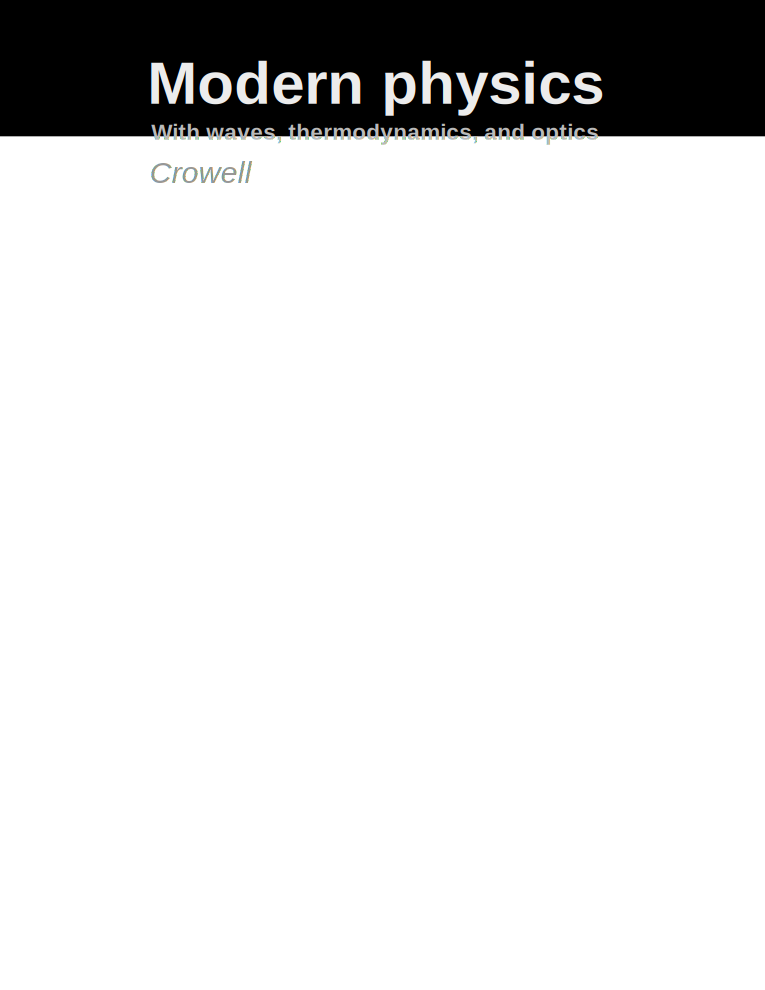
\includegraphics{\chapdir/figs/cover}\\
}
}%
\\


\end{titlepages}

\begin{titlepages}[2]
  \brieftitle
\end{titlepages}

\begin{titlepages}
  \copyrightpage{2019}
  \vspace{100mm}
  \noindent\emph{About the cover:} The cover shows a simulated image of the sky as viewed by an observer who has fallen into a black hole.
  The constellations Orion and Canis Major are visible. Although the observer is already inside the event horizon, the bending
  of light rays by gravity makes it appear as though the black hole only occupies a relatively small part of the field of view.
  The bright ring consists of light from
  stars that are not actually very bright. Their light is amplified because they happen to lie near the event horizon.
  The image was rendered by the open-source library Karl, \url{github.com/bcrowell/karl}. 
  \vfill
\end{titlepages}

\normalsize\normalfont\pagebreak\thispagestyle{empty}\cleardoublepage\thispagestyle{empty}

\yesiwantarabic
\nomarginlayout
\vspace{10mm}\begin{center}\bfseries\sffamily{}\noindent{}{\huge Brief Contents}\end{center}\vspace{10mm}

\newcommand{\brieftocpartstyle}{\large\sffamily{}}
\newcommand{\brieftocchstyle}{\normalsize\sffamily{}}
\newcommand{\brieftocvert}{7mm}
\newcommand{\brieftochoriz}{\hspace{20mm}}
\newcommand{\brieftoctabularwidth}{90mm}

\vspace{\brieftocvert}\noindent\brieftochoriz%
\brieftocchstyle\begin{tabular}{rp{\brieftoctabularwidth}}
& \textit{\brieftocpartstyle Waves and relativity}\\
\brieftocentry[\hfill]{ch:time}{Time} \\
\brieftocentry[\hfill]{ch:waves}{Waves} \\
\brieftocentry[\hfill]{ch:em-waves}{Electromagnetic waves} \\
\brieftocentry[\hfill]{ch:lorentz}{The Lorentz transformation} \\
\brieftocentry[\hfill]{ch:media}{Waves done medium well} \\
\brieftocentry[\hfill]{ch:rel-dynamics}{Relativistic energy and momentum} \\
& \textit{\brieftocpartstyle Thermodynamics}\\
\brieftocentry[\hfill]{ch:stat}{Statistics and the ideal gas} \\
\brieftocentry[\hfill]{ch:macro}{The macroscopic picture} \\
\brieftocentry[\hfill]{ch:entropy}{Entropy} \\
\end{tabular}




\onecolumn\vfill
\mynormaltype

\pagebreak[4]

\vspace{0mm}
\begin{center}
\noindent\huge\bfseries\sffamily{}Contents\mynormaltype
\end{center}
\vspace{0mm}
\begin{multicols}{2}
  \tableofcontents
  \setcounter{unbalance}{0}
\end{multicols}
\normallayout\onecolumn

%========================= main matter =========================
\mainmatter
%-- I want the whole book numbered sequentially, arabic:
  \pagenumbering{arabic} 
  \addtocounter{page}{8}
\parafmt
\myeqnspacing % Do this early and often, since it gets reset by \normalsize
%========================= chapters =========================
\wugga%used to be needed after preface
    \renewcommand{\chapdir}{waves}\include{waves/atemp}
    \renewcommand{\chapdir}{waves}\include{waves/btemp}
    \renewcommand{\chapdir}{waves}\include{waves/ctemp}
    \renewcommand{\chapdir}{waves}\include{waves/dtemp}
    \renewcommand{\chapdir}{waves}\include{waves/etemp}
    \renewcommand{\chapdir}{waves}\include{waves/ftemp}
    \renewcommand{\chapdir}{thermo}\include{thermo/atemp}
    \renewcommand{\chapdir}{thermo}\include{thermo/btemp}
	\formatchtoc{\large}{\quad\contentspage}{4mm} % This has to go before the last chapter.
    \renewcommand{\chapdir}{thermo}\include{thermo/ctemp}
        \addtocontents{toc}{\vspace{5mm}}% For reasons I don't understand, this actually comes *after* the final chapter.
%
    \widelayout
    \renewcommand{\chapdir}{end}
    \include{end/skillstemp}
    \onecolumn\include{end/hwanstemp}
    \include{end/mathtemp}
    \onecolumn\include{end/photocreditstemp}
%========================= index =========================
\label{splits:index}\printindex
%========================= data tables, etc. =========================
        \blankchaptermarks\label{splits:data}
        \input{end/data}

\end{document}
